\section{Customisation}

Users are given several options in the settings to customise their experience. The majority of these settings are given to allow the user to customise the level of real-time feedback that they receive. They can choose any combination of repetition counting, vocal feedback and tips, vocal instructions to direct them, and beeps to indicate detection and that they have descended low enough. Figure~\ref{fig:settings} shows part of the scrollable settings page.

\begin{figure}[H]
    \centering
	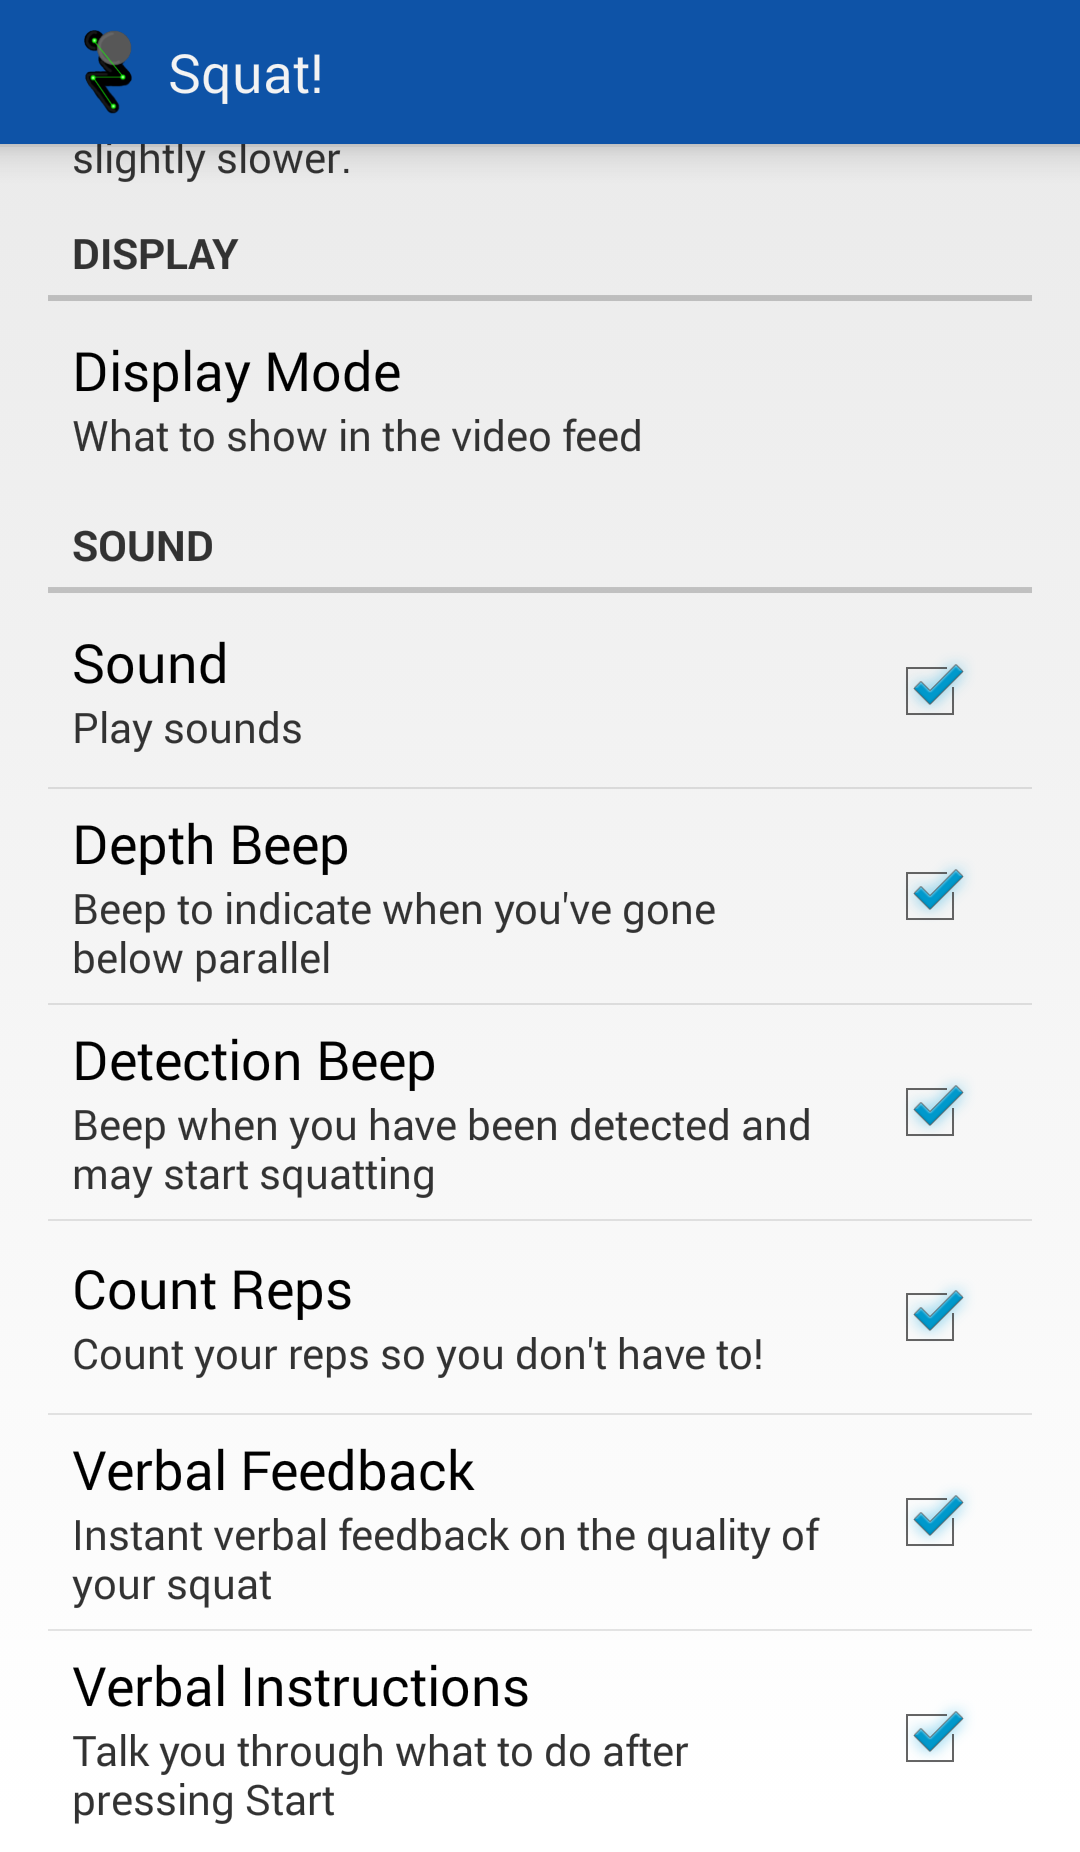
\includegraphics[height=10cm]{application/images/settings}
\caption{A screenshot of the settings menu of the application}
\label{fig:settings}
\end{figure}

The user is also given the ability to customise the detection stage of the algorithm, setting the detection's motion sensitivity and detection time. The motion sensitivity dictates how still the lifter must be in order to be detected and for the initial model fit. The detection time dictates how long the lifter must stand still before the model is mapped to them and they can begin squatting. This customisation allows the user to choose whether they prefer to walk out and start squatting quickly, or whether they would rather take a little longer to get into position and adjust their foot placement.

The user is also given a `Squatting With Barbell' checkbox. This allows the user to select whether or not they are squatting with a weight on their back, and the model will draw the weight on its shoulders if selected. This allows the user to practice squatting without a barbell, and gives better tracking results for that case.

Settings are implemented using Android's Preferences API, which ensures that changes made to the settings persist with no explicit use of a database.